\documentclass[10pt]{beamer}

\usepackage{ucs}
\usepackage[utf8x]{inputenc}
\usepackage{beamerthemeshadow}
\usepackage{amsmath}
\usepackage[british]{babel}
\usepackage{fontenc}
\usepackage{graphicx}
\usepackage{tikz}
\usetikzlibrary{arrows,positioning}
\usetikzlibrary{shapes,snakes}

\title{An Introduction to Python}
\author{William Vigor and Cylde Fare}
\date{}
\newcommand{\bra}[1] { \langle #1 | }
\newcommand{\ket}[1] { | #1 \rangle }
\newcommand{\bket}[1] { \langle #1  \rangle }
\newcommand{\brket}[2] { \langle #1 | #2 \rangle }
\newcommand{\braket}[3] { \langle #1 | #2 | #3 \rangle }
\newcommand{\ketbra}[1] {\ket{#1}\bra{#1}}
\begin{document}

\maketitle
\titlegraphic{
\includegraphics[width=0.5\textwidth]{Imperial_2_Pantones.pdf}
}
\frame{
        \frametitle{Philosophy of the Course}
\begin{itemize}
\item Hands on: only this short introductory talk. No one wants to listen to lectures about how to program.
\item 3 Workshops:
\end{itemize}
\begin{enumerate}
\item Introduction: the basics of python. How to write a simple program.
\item Using python for science.
\item Advanced python.
\end{enumerate}


}
\part{Introduction: What is Programing ?}
\frame{\partpage}


\frame{
        \frametitle{What is programing ?}
\begin{itemize}
\item A Computer Program :
\end{itemize}
``A sequence of instructions that a computer can interpret and execute "
\begin{itemize}
\item In scientific programing these instructions can are used to either anaylise expremantal data or for computational simulation. 
\end{itemize}

\begin{itemize}
\item Scientific simulations run on many of the fastest computers in the world. (10,000's of CPUs)
\end{itemize}


\begin{figure}
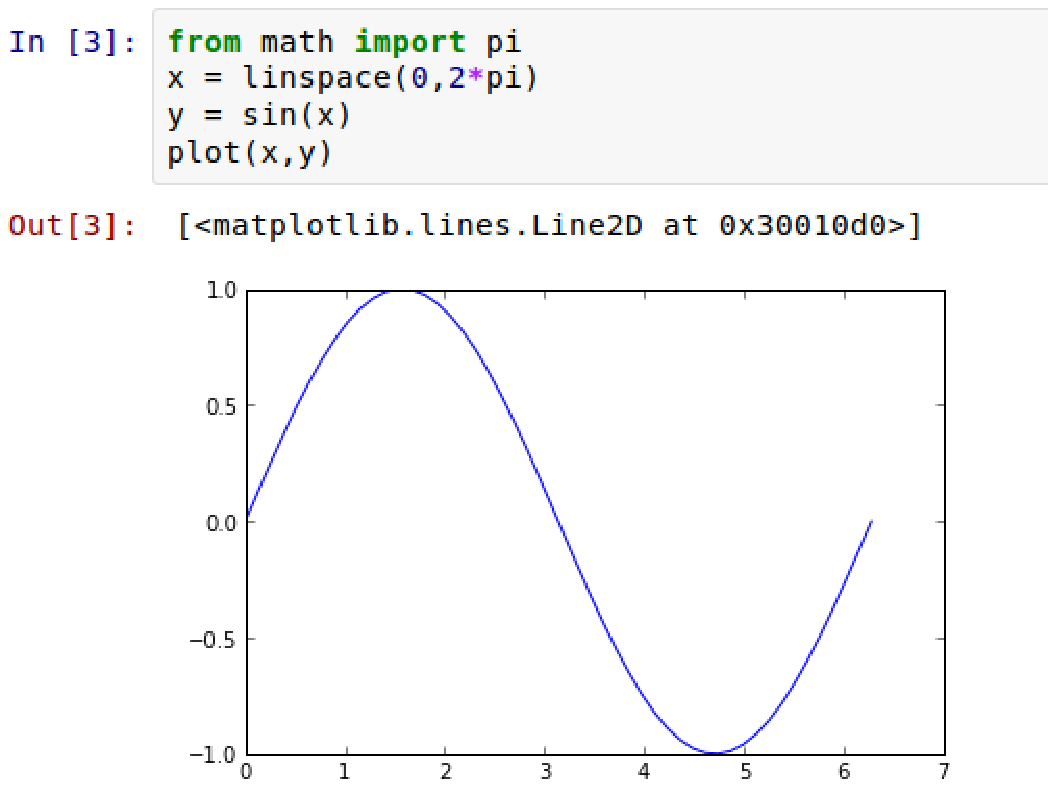
\includegraphics[width=0.5\textwidth]{sinx.pdf}
\end{figure}


}


\frame{
        \frametitle{Why Programming is Hard}
\begin{itemize}
\item Computers are dumb. (They simply follow instructions logically however stupid the instruction may be).
\item Computers have no empthy.
\end{itemize}
`` Computers are good at following instructions, but not at reading your mind. " 
Donald Knuth 

``As soon as we started programming, we found to our surprise that it wasn’t as easy to get programs right as we had thought. Debugging had to be discovered. I can remember the exact instant when I realized that a large part of my life from then on was going to be spent in finding mistakes in my own programs."
Maurice Wilkes (1949)
}

\frame{
        \frametitle{Why Learn to program}
\begin{itemize}
\item Experimental equipement is now commonly computerised.
\item A powerful tool to anaylise experimental data more efficeintly.
\item Write computer simulations to complement experimantal data.
\item A usefull transferable skill.
\end{itemize}

}

\frame{
        \frametitle{Why Learn to program}
\begin{itemize}
\item Make science reproducable:
\item A program ran once with the same inputs should produce the same results if ran again.
\end{itemize}
}


\part{Why Python ?}
\frame{\partpage}

\frame{
	\frametitle{Python Versus other Lanuagues}
\begin{itemize}
\item Easy to learn but powerful.
\item Python's syntax is designed to be readable (compared to perl for example).
\item No need to worry about memory allocation/deallocation (e.g. in C).
\item Easy to run no need for compliation.
\end{itemize}
}
\frame{
	\frametitle{Python Versus other Lanuagues}
\begin{itemize}
\item Batteries included: No need to reinvent the wheel:
\item Many opensource scientific and other libaries avaiable.
\item e.g. Matplotlib
\end{itemize}
\begin{figure}
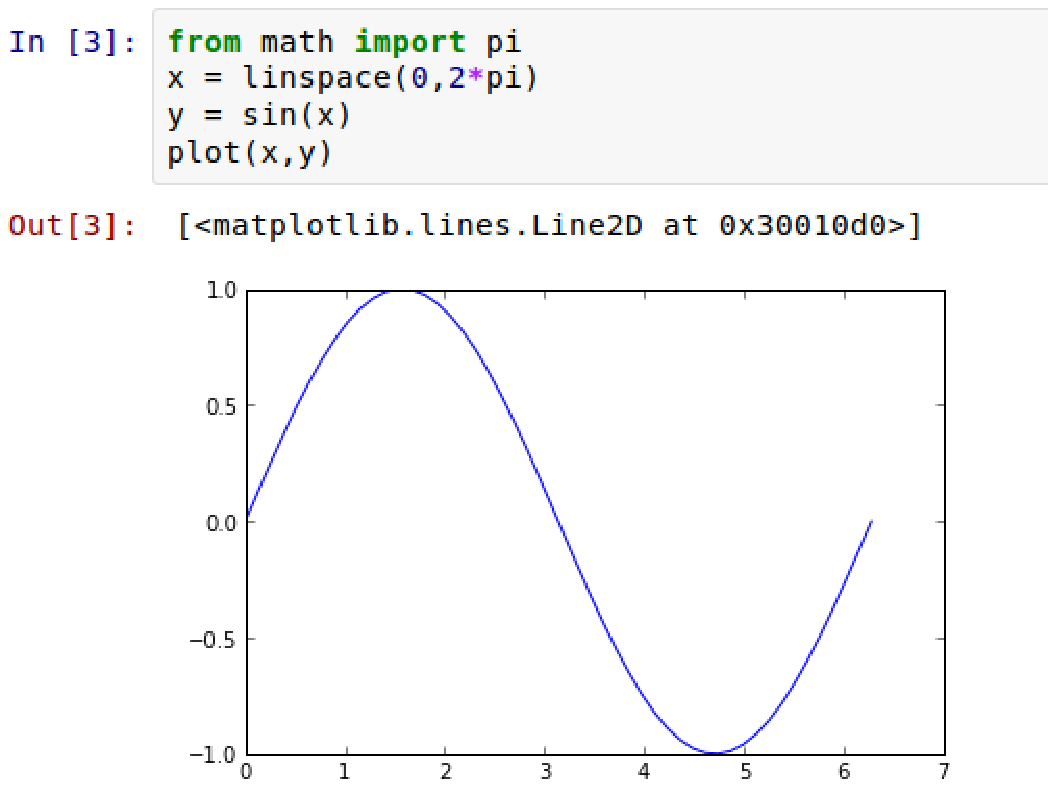
\includegraphics[width=0.5\textwidth]{sinx.pdf}
\end{figure}
}




\frame{
	\frametitle{Python is Opensource}

\begin{itemize}
\item No need to buy a license, can use it at home even after you leave Imperial.
\item Compatatble across multiple platforms Linux, Mac, Windows.
\item A large group of people are interested in developing new features.
\item If a feature is not present then you can add it in yourself might be useful for others.
\item You can look at the code to check it is doing what you think it's doing.
\end{itemize}
}


\part{How to can we run Python}
\frame{\partpage}
\frame{
	\frametitle{From the Command Line}
\begin{itemize}
\item Put python code into .py file using a text edditor.
\item Run on the command line: python test.py 
\end{itemize}
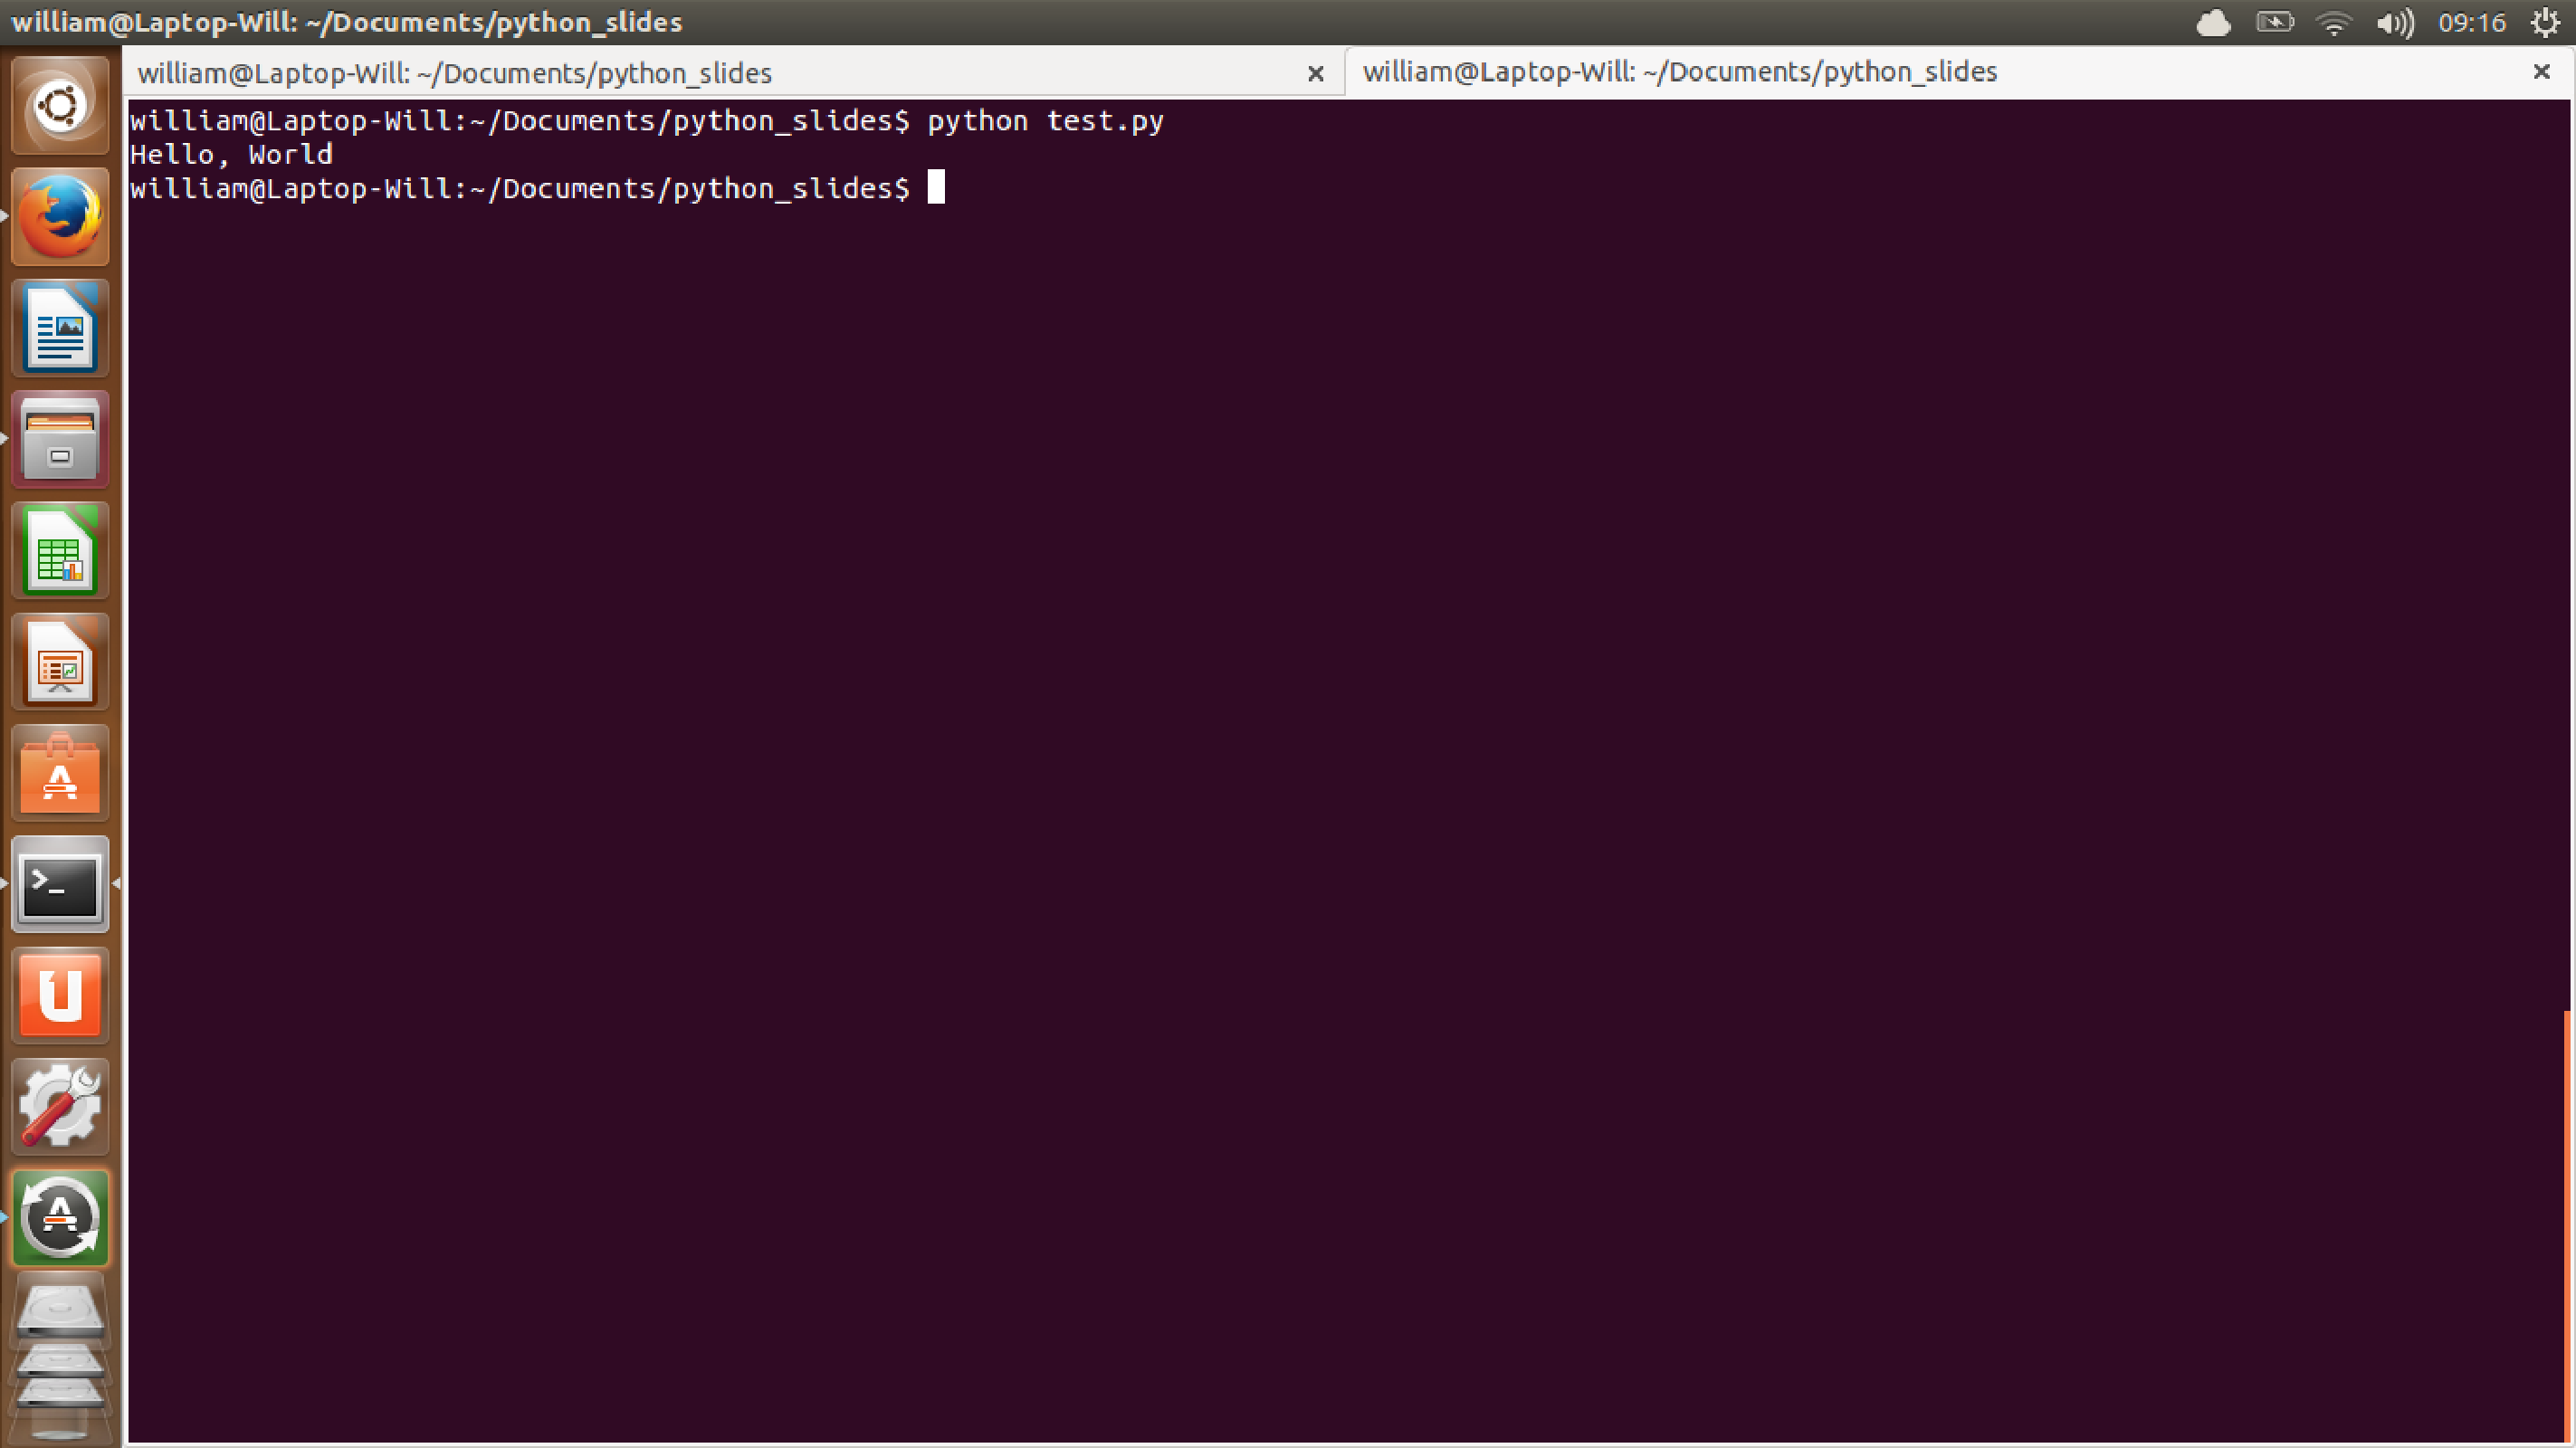
\includegraphics[width=0.5\textwidth]{term.pdf}
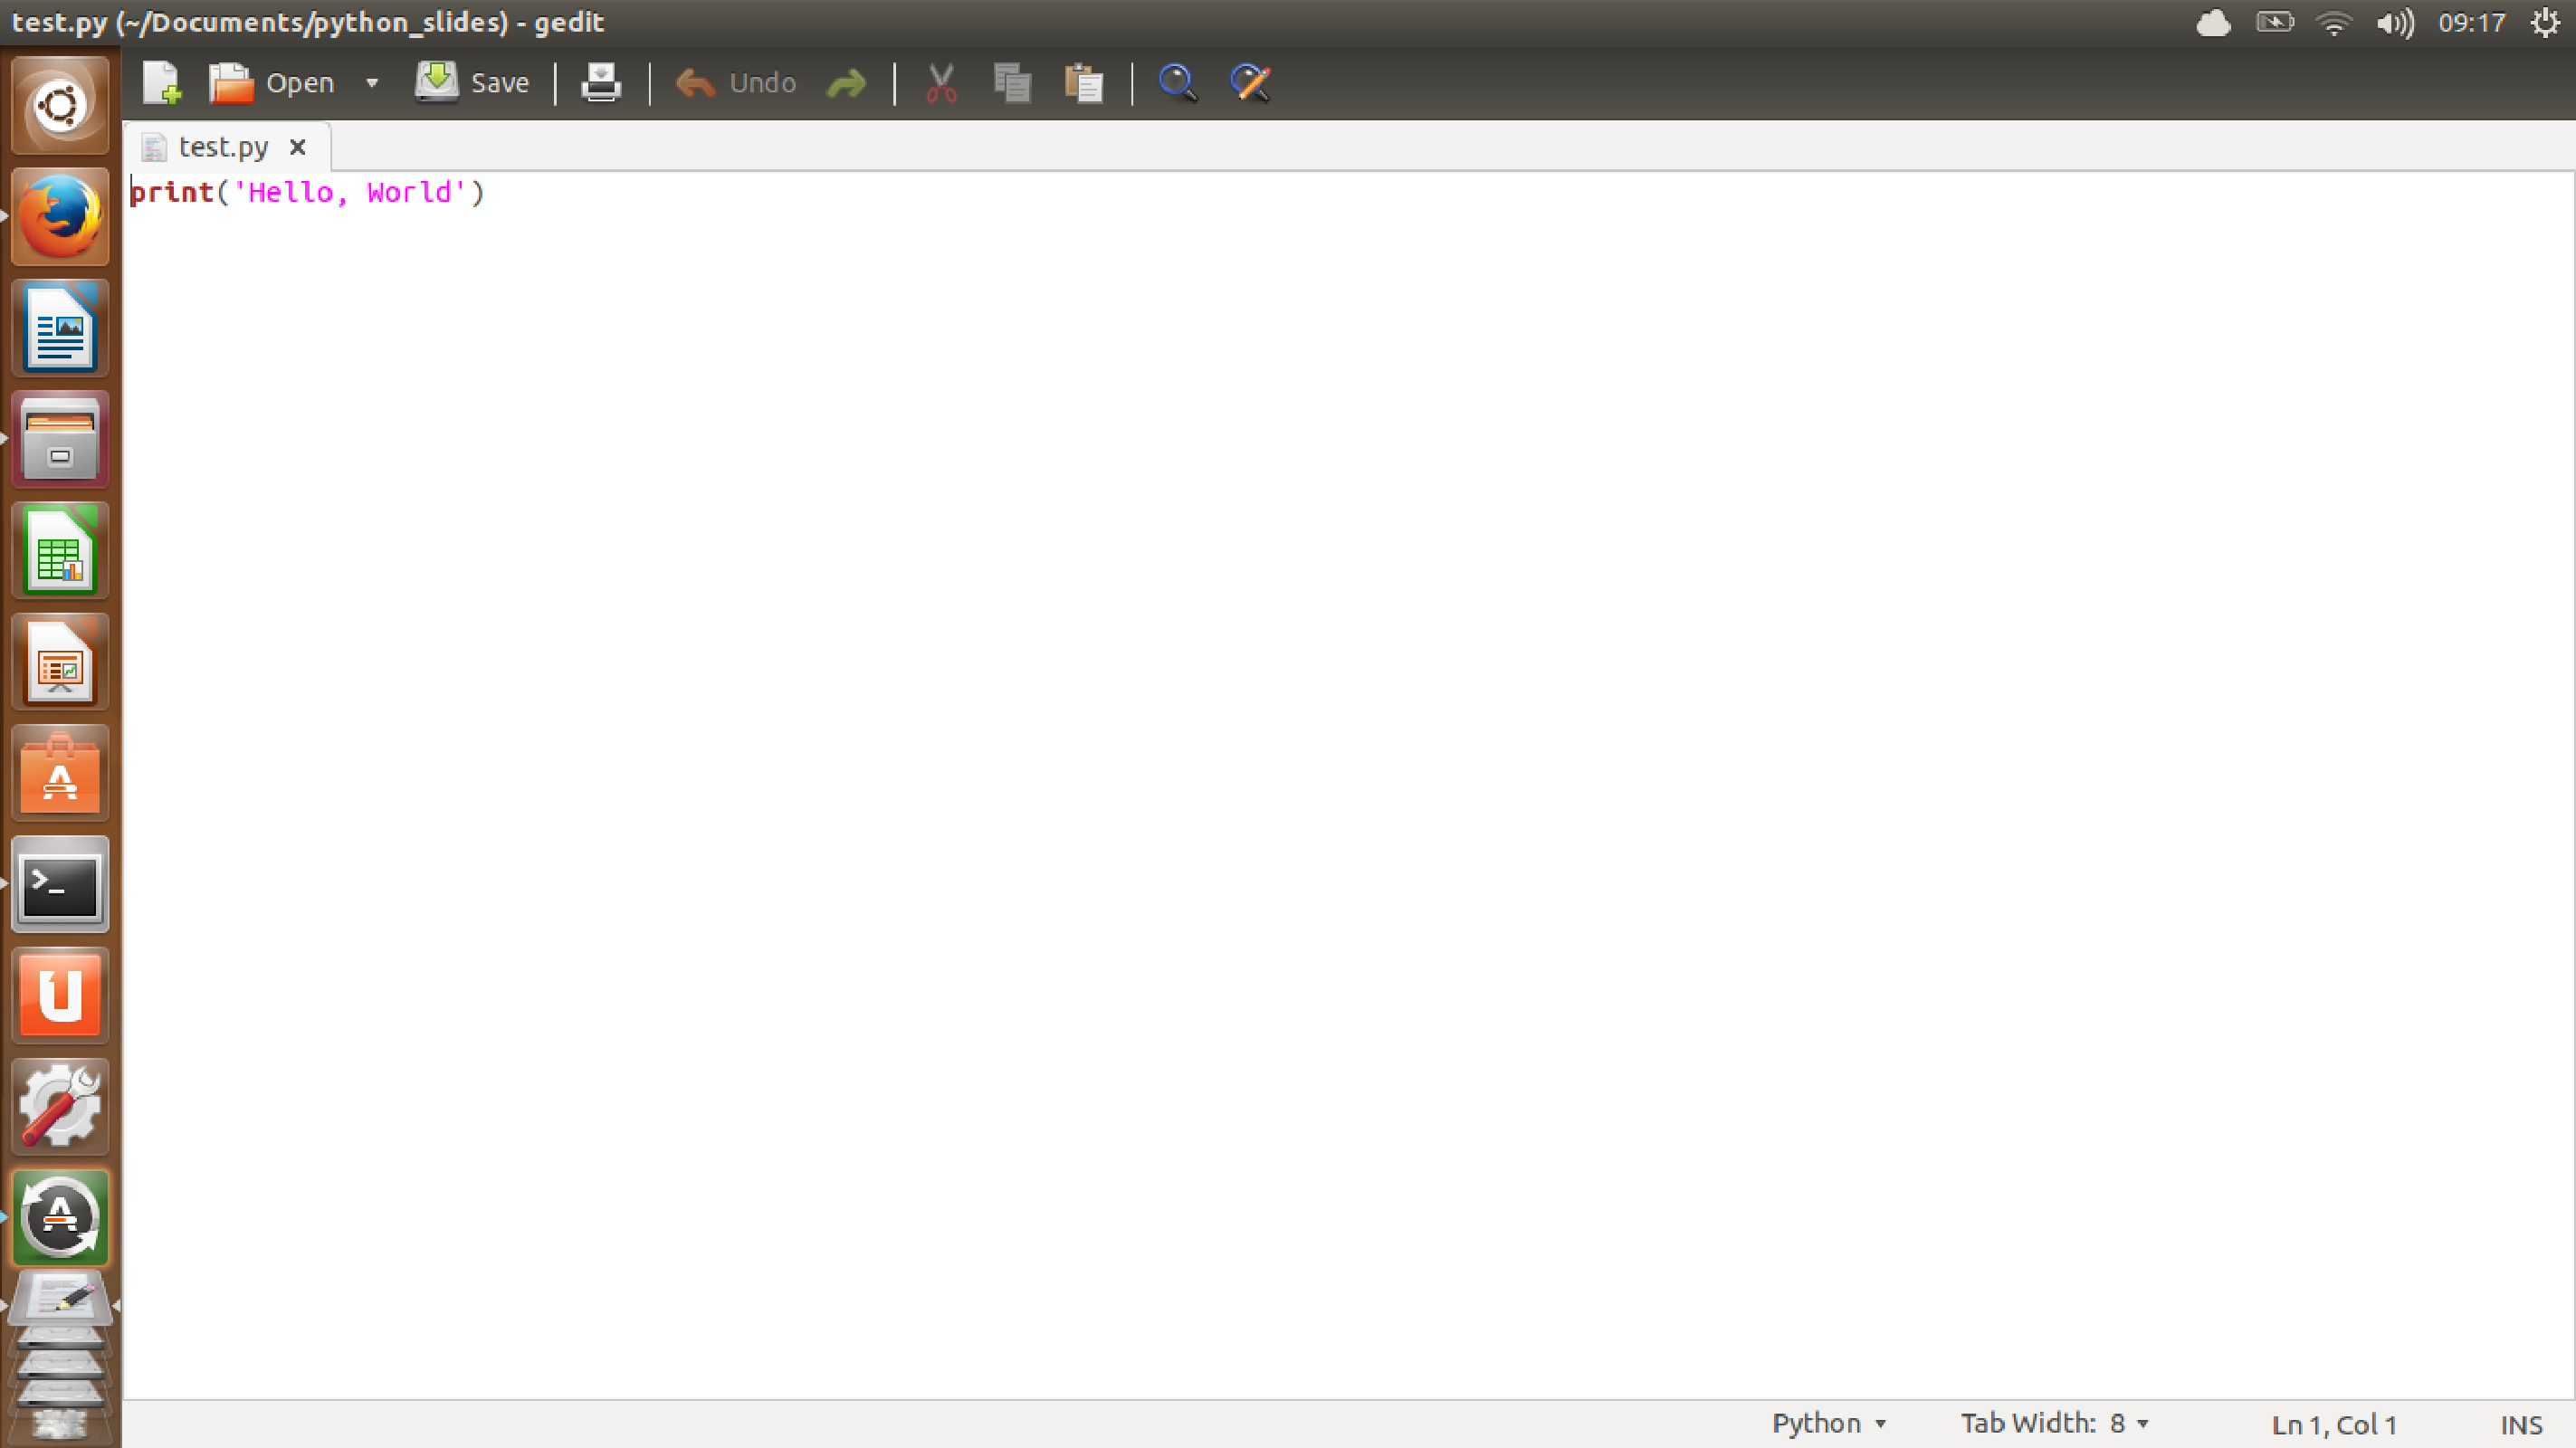
\includegraphics[width=0.5\textwidth]{file.pdf}
\begin{itemize}
\item Usefull for scripts and finished programs.
\end{itemize}
}
\frame{
	\frametitle{Using the ipython Interactive enviroment}

\begin{itemize}
\item To launch from the command line: ipython
\item Interactive session consists of a number of cells which are ran cosetutively.
\end{itemize}
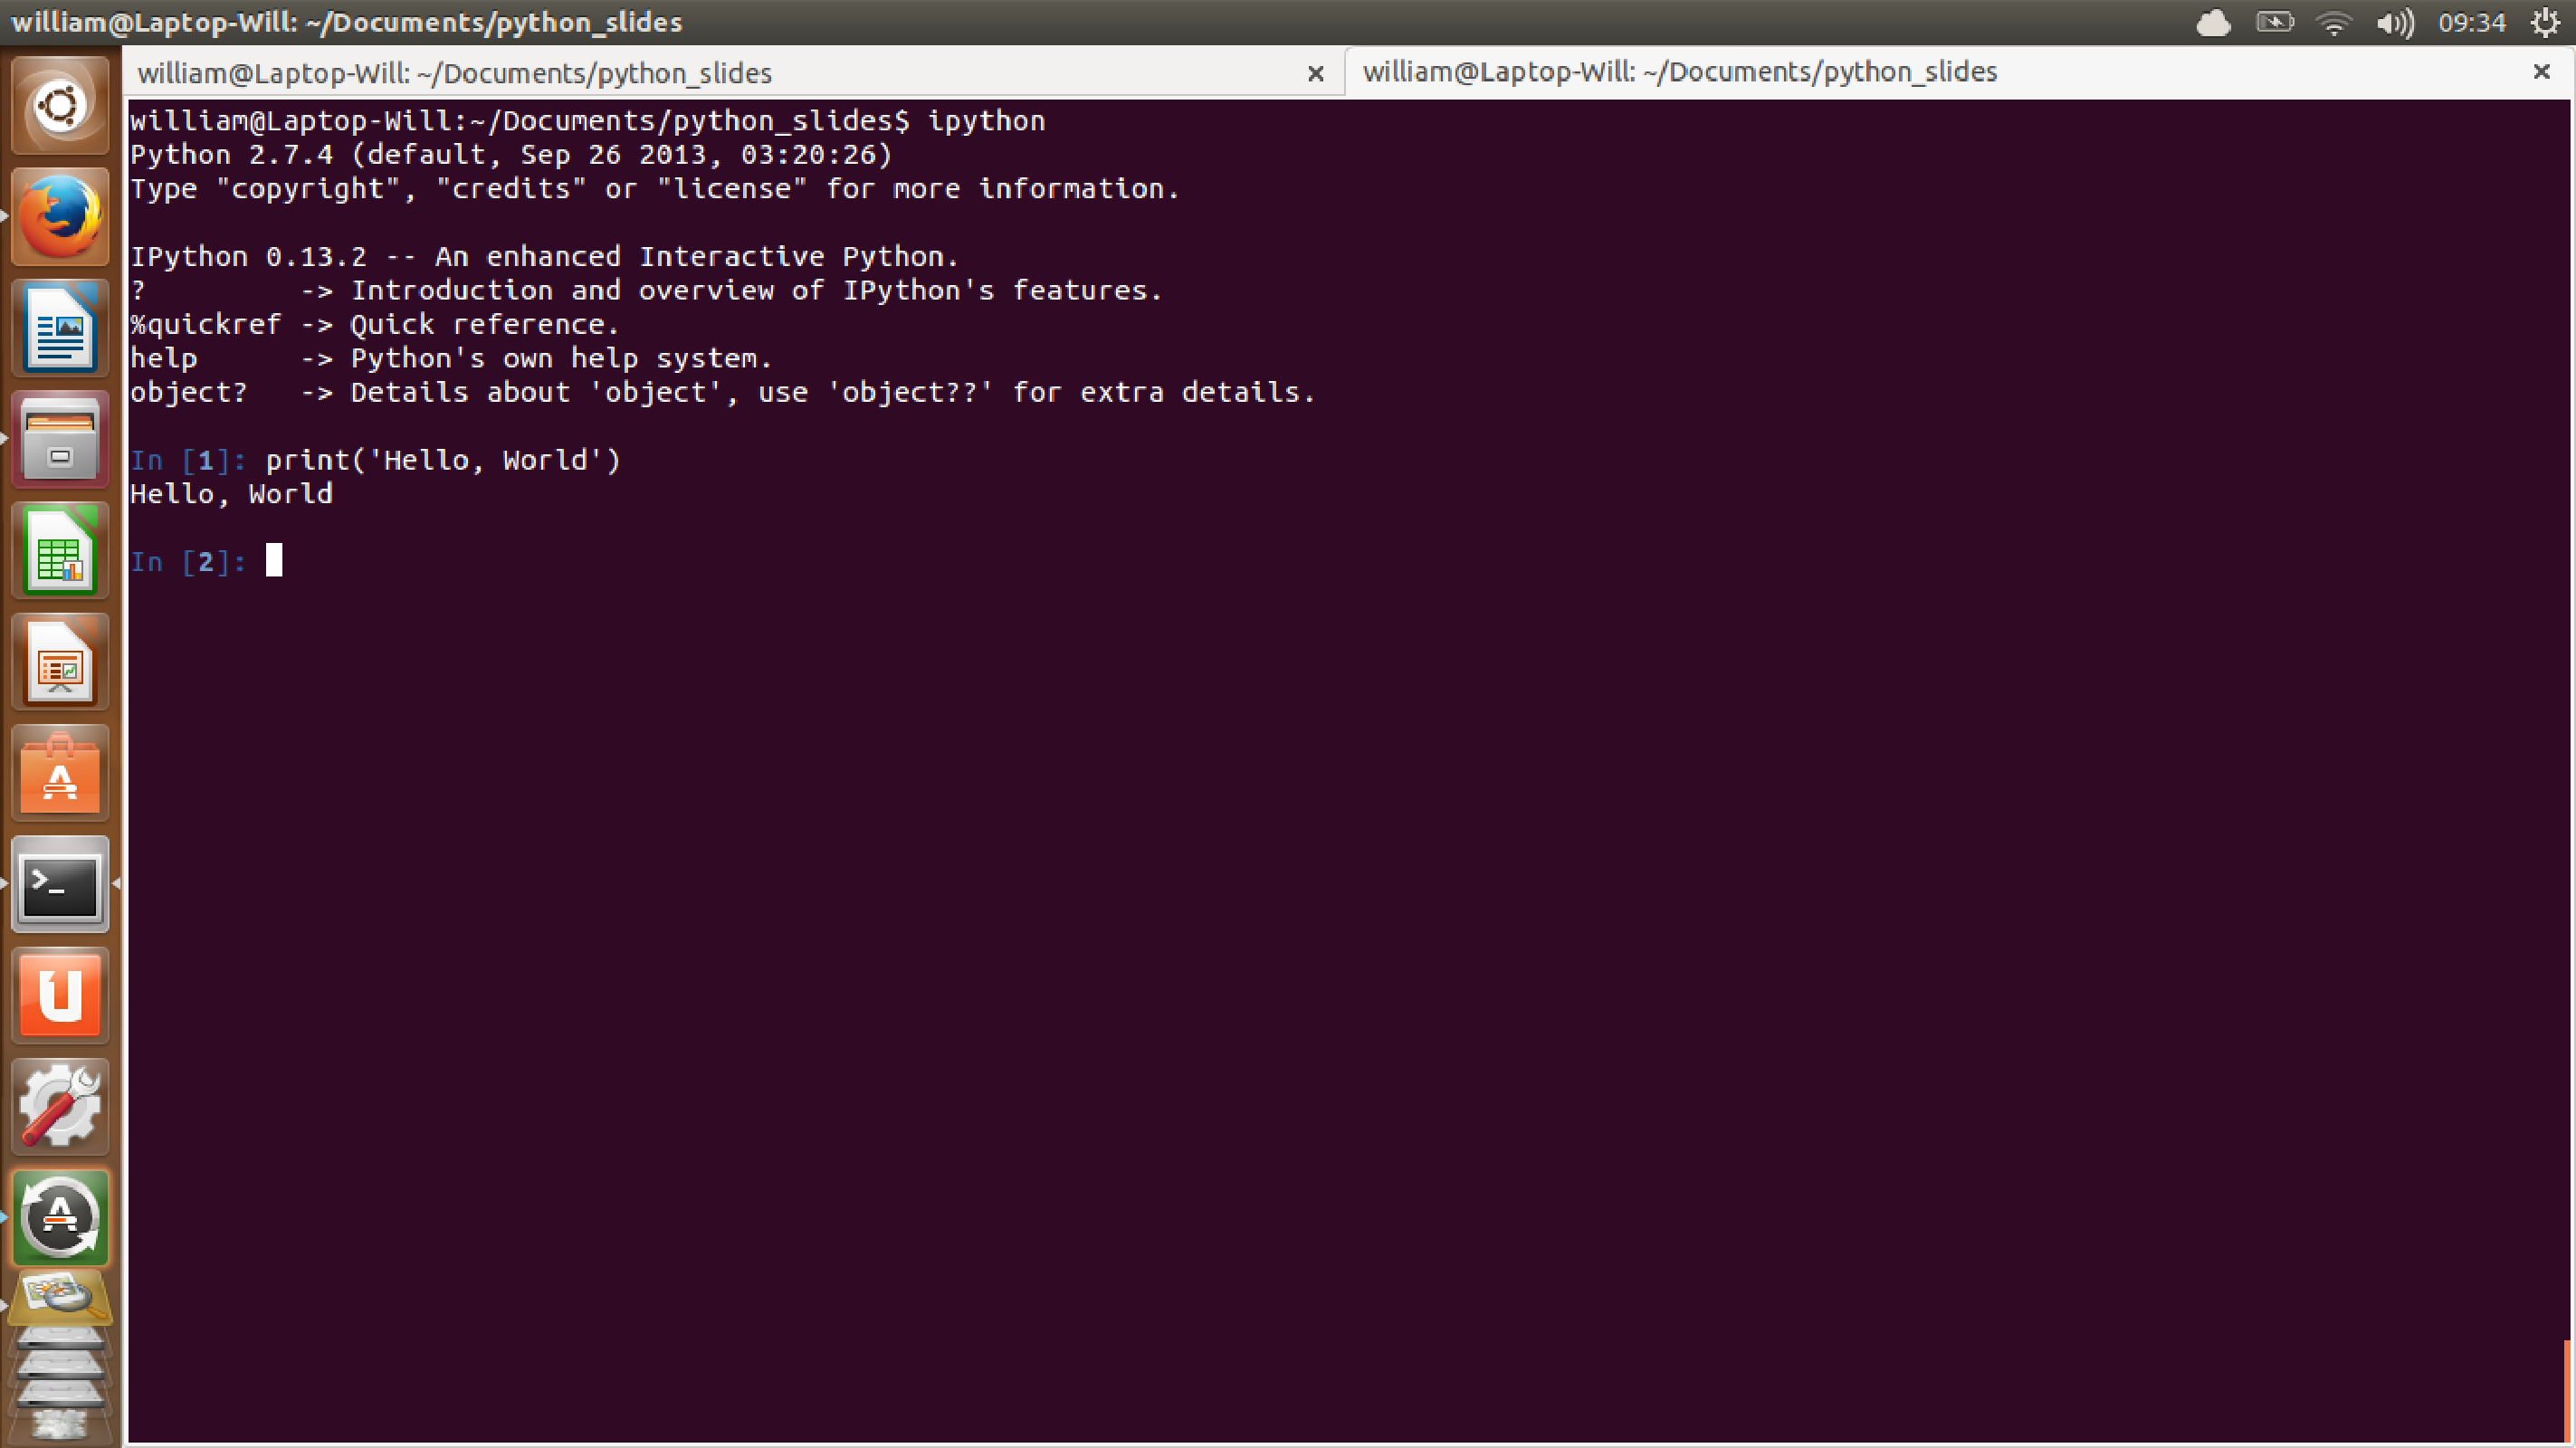
\includegraphics[width=0.5\textwidth]{ipython.pdf}

\begin{itemize}
\item Usefull for quickly testing out simple ideas which can be put into a .python file later.
\item Unfortunatly once ipython is closed the code is lost.
\end{itemize}
}
\frame{
	\frametitle{Using the ipython Interactive Notebook}

\begin{itemize}
\item To launch from the command line: ipython notebook --pylab=inline
\item Interactive session consists of a number of cells which can be ran in any order.
\item Can insert plain text and latex for extra notes.
\end{itemize}
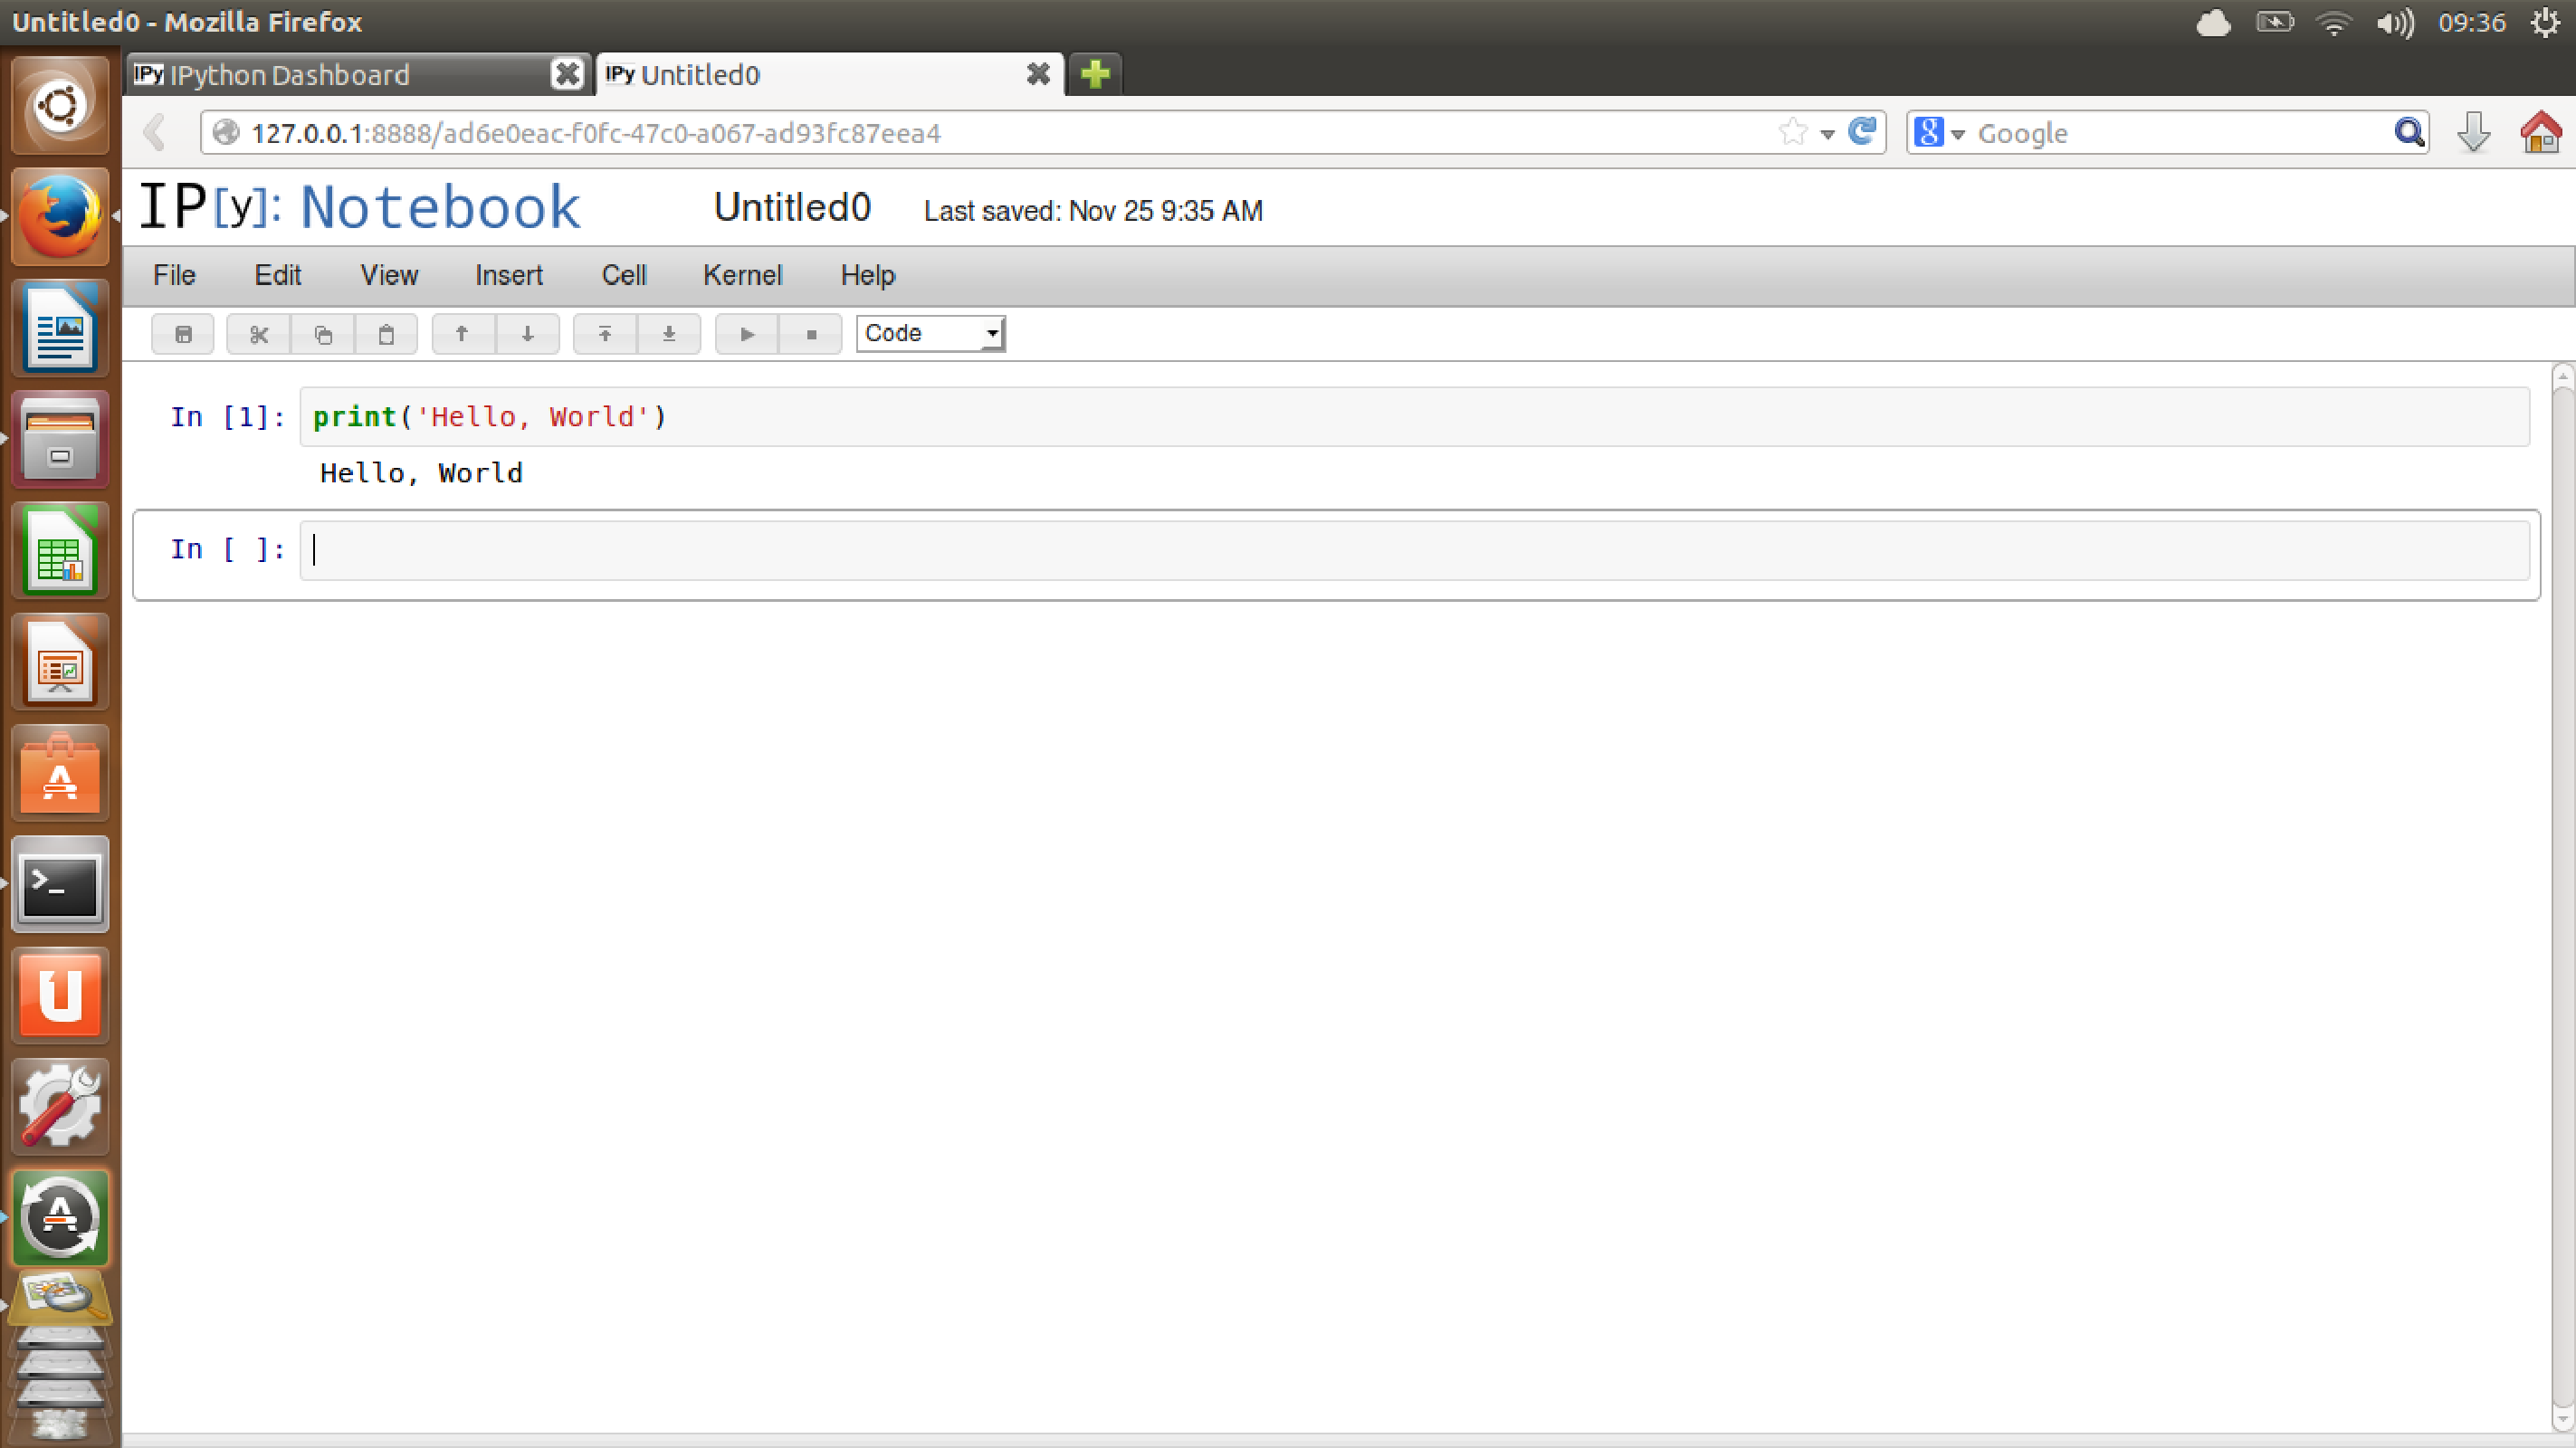
\includegraphics[width=0.5\textwidth]{ipython-notebook.pdf}
}
\frame{
	\frametitle{Using the ipython Interactive Notebook}
\begin{itemize}
\item Can be used to make a Lab Notebook to anaylise data.
\item Graphs generted from the code can be directly placed into the notebook.
\end{itemize}
}
\frame{
	\frametitle{Other Resources}

\begin{itemize}
\item General python: \href{http://doc.python.org/2/}{http://doc.python.org/2/}
\item Scipy: \href{www.scipy.org}{www.scipy.org}
\item Numpy: \href{www.numpy.org}{www.numpy.org}
\item Further tutorials: 
\item Anaconda distrubution: \href{https://store.continuum.io/cshop/anaconda/}{https://store.continuum.io/cshop/anaconda/}
\end{itemize}
}

\frame{
	\frametitle{Tips}
\begin{itemize}
\item Write code which is easy to read. (Code should be written for Humans not computers)
\item The simplest solution to a problem is almost always the best.
\item Ask questions. It is easy to have misconceptions about programing.
\end{itemize}
}
\end{document}
